\documentclass[12pt, a4paper]{report}
\usepackage{lmodern}
\usepackage[T1]{fontenc}
\usepackage[czech]{babel}
\usepackage[utf8]{inputenc}
\usepackage{graphicx}
\usepackage{hyperref}
\usepackage{listings}
\hypersetup{
	colorlinks=true,
	linkcolor=black,
	urlcolor=blue
}
\begin{document}
\author{Jan Strnádek}
\date{10.10.2012}
\title{KIV/PRJ5\\SID\\\small{SQL Injection Detector\\Tento program je určen pouze k školním a testovacím účelům! Je zakázáno ho využívat k nelegální činnosti a autor ani ZČU nenese jakoukoliv zodpovědnost škodám způsobeným využitím softwaru a ani jeho součástí pro nelegální účely}}
\begin{titlepage}
\begin{center}
\textsc{\Large Západočeská Univerzita v Plzni}
\\[0.3cm]
\textsc{\Large Fakulta Aplikovaných Věd}
\\[0.3cm]
\textsc{\Large Katedra Informatiky a výpočetní techniky}
\\[6cm]
\textbf{\LARGE Bakalářská Práce}
\\[3cm]
\textbf{\LARGE SID\\[0.3cm] Sql Injection Detector}
\\[7cm]
\begin{minipage}{0.4\textwidth}
\begin{flushleft}
\large
Plzeň, 2013
\end{flushleft}
\end{minipage}
\begin{minipage}{0.4\textwidth}
\begin{flushright} 
Jan Strnádek
\end{flushright}
\end{minipage}
\vfill
\end{center}
\end{titlepage}
\tableofcontents
\chapter{Úvod}
V dnešní době je internet synonymem pro používání počítače, tabletu, smartphone a jiných zařízení. S tím rozhodně souvisí otázka bezpečnosti uživatelských dat. Většina uživatelů bohužel využívá jedno stejné heslo a to všude, proto obezřetnému hackerovi stačí získat email a heslo z jedné databáze a zkusit to i jinde. Situace, která se stala nedávno při hacku pornostránek skupinou \uv{LulzSec}\footnote{Lulz Security - tato skupina stála i za útokem na Sony Pictures v roce 2011, kde právě díky SQL Injection odcizila velké množství dat.}, tato skupina následně data zveřejnila (hesla nebyla v DB nijak \uv{hashována}\footnote{Hash - algoritmus pro převedení vstupních dat do unikátního otisku, tato funkce \uv{by měla být jednosměrná!}}, byla uložena normálně) a proto nebyl problém vyzkoušet se přihlásit do emailových schránek, popřípadě dalších jiných webových služeb, kteří tito uživatelé využívali. Nikdy přesně nevíme komu vlastně  data svěřujeme a jaké bezpečnostní opatření je dotyčnou firmou či osobou zajištěno! Data jsou uchováváná v mnoha databázových systémech a jednou z hlavních otázek je také bezpečnost těchto dat. Možností útoků na webové applikace, webové stránky nebo přímo servery je mnoho. Příkladem mohou být:
\begin{itemize}
\item SQL Injection - normal / blind
\item XSS - Cross-Site scripting - local / persistent (stored) / non-persistent (reflected)
\item CSFR - Cross-Site Request Forgery 
\item DT - Directory traversal
\item PHP remote upload and execution scripts
\item a mnoho dalších, protože webový server je pořád server s operačním systémem, který již v základu nějaké chyby obsahuje.
\end{itemize}
Tato práce je zaměřena na detekci prvního zmíněného problémů a to je SQL Injection. Aktuálně je podle serveru \uv{http://techworld.com} je za zhruba 97\% úniky dat právě zneužití této chyby. Se zajímavými daty přichází i server \uv{http://cnet.com}, který uvádí, že každé 2 minuty je atakována nějaká webová stránka a to s následujícími typy:
\begin{itemize}
\item 37\% - Directory traversal
\item 36\% - Cross Site Scripting
\item 23\% - SQLi
\item 4\% - remote file inclusion
\end{itemize}

\section{XSS - Cross-Site scripting}
XSS využívá podobně jako SQLi neochráněných vstupních proměnných na webových stránkách. Díky nim může do aplikací podstrčit svůj vlastní (například JavaScriptový) kód, což může následně využít k získání dat (zejména cookies od uživatelů), znedostupnění webových stránek atd. Existují dva základní typy XSS útoku:

\subsection{Nepersistentní}
Tento typ využívá nezabezpečených vstupních proměnných z URL adresy / POST dat, které jsou vypisovány na stránku. Útočníkovi stačí URL upravit a nějakým jiným způsobem (například sociálním inženrstvím, podvrženým emailem z banky apod.) donutit uživatele na tento okdaz kliknout. 

\subsection{Persistentní}
Tento typ je mnohem nebezpečnější protože na napadné stránky se nevstupuje přes upravenou URL adresu, ale kód se vykonává automaticky (tato chyba se často objevuje v různých diskusních fórech, návštěvních knihách, kde se nevalidují vstupy). Do těch těchto nezabezpečených vstupů stačí pouze účtočníkovi vložit JS kód, který se následně provede každému, kdo tuto stránku otevře. 

\subsection{Ukázka}
Na obrázku \ref{obr.airbank} můžeme vidět úspěšný nepersistentní XSS útok na serveru air/bank. V nechráněném vstupu byl zadán kód výstražné hlášky javascriptu:
\begin{center}
\textit{<script type="text/javascritpt"$>$alert("XSS by PiratezSec");</script>}
\end{center}
Tato chyba byla objevena skupinou Czechurity, která má na svědomí i hacknutí webových stránek Unicredit bank v březnu 2013, které bylo médii chybně interpretováno jako DDoS\footnote{Distributed Denial of Service - útok, který zahlcuje službu pro pád nebo nedostupnost pro ostatní uživatele.}.
\begin{figure}
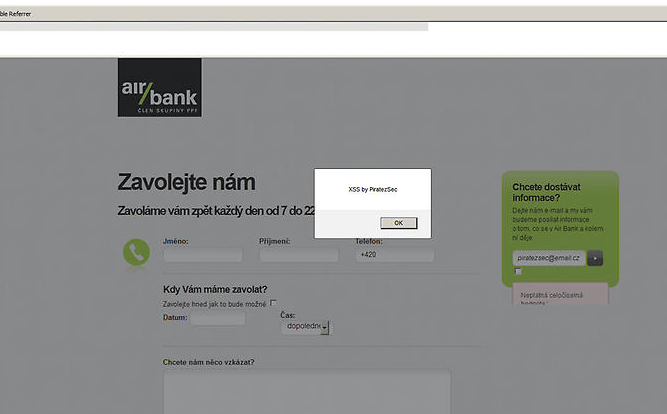
\includegraphics[width=390px]{./examples/xss-airbank.png}
\caption{Non-persistent XSS}
\label{obr.airbank}
\end{figure}

\subsection{Různé varianty zapsání XSS}
Výstupy na různých webových stránkách mohou být různým způsobem filtrovány, popřípadě může být přímo filtrován script tag, lze toto obejít? Odpovědí je bohužel ano, možné to je a je to značně jednoduché, zde několik příkladů:

\begin{itemize}
\item Schování javascriptu do neexistujícího obrázku: \textit{<img src="javascript:alert('XSS');">}
\item Zakázané uvozovky? není problém \textit{<img src=javascript:alert(\&quot;XSS\&quot;)>}
\end{itemize}

\subsection{Obrana}
Obrana před XSS není snadná, velké webové portály mají desítky různých vstupů a ty všechny se musí hlídat. Ideální obranou je pokud se rozhodneme využít nějaký framework, tak vybereme ten jehož předností je právě těmto incidentům předcházet (Nette, RoR apod.). Nebo proti persitentním útokům hlídat co ukládáme do databáze popřípadě do jiných úložišť.


\section{Directory traversal}
Webový server slouží hlavně pro \uv{servírování} souborů, soubory mohou být statické (obrázky, css styly, HTML soubory) nebo dynamické (Ruby, PHP, ASP atd.). Pokud vytvoříme požadavek na web server server nám při statickém obsahu soubor okamžitě vrací, při dynamickém ho nejdříve zpracuje a následně vrátí. Při útoku typu \uv{direcotry traversal} využívá útočník špatného (žádného) omezení přístupu k souborům přes webový server.

\subsection{Příklad directory traversal útoku}
Mějme URL adresu:
\begin{center}
\textit{http://portal.czu.cz/index.php?item=novinky.html}
\end{center}
název souboru \uv{novinky.html} nám naznačuje, že by mohlo jít o vložení obsahu souboru \uv{novinky.html} odněkud ze souborového systému do stránky. Otázkou však zůstává co se bude dít, budeme-li tento parametr měnit ručně? a kam až se dostanem?
\begin{center}
\textit{http://portal.czu.cz/index.php?item=../.htaccess}\\
Pokus o získání \.htaccess souboru
\newline
\textit{http://portal.czu.cz/index.php?item=../config/config.neon}\\
Pokus o získání neon souboru na webech využívající Nette\footnote{Nette Framework - Framework sloužící pro zajištění MVC architektury v PHP aplikacích, v config.neon jsou uložena přístupová data k databázím a další nastavení.}
\end{center}

\subsection{IIS Web Server}
Starší verze IIS\footnote{Internet Information Service - web server od společnosti Microsoft} umožňovaly dokonce i vykonávat soubory na serveru!

\begin{center}
\textit{http://iis.czu.cz/scr/..\%5c../winnt/system32/ cmd.exe?/c+dir+c:$\backslash$}
\end{center}

Tento příkaz spustil \uv{cmd.exe}\footnote{Příkazová řádka systému Windows} a v něm příkaz \uv{dir c:$\backslash$}. Nic nám tedy nebrání přidávat uživatele do systému, nebo formátovat pevné disky.

\subsection{Praktická ukázka}
\begin{figure}[h!]
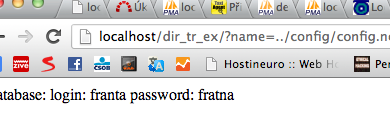
\includegraphics[width=390px]{./examples/dir_example.png}
\caption{Directory traversal - zobrazení souboru config.neon}
\label{obr.airbank}
\end{figure}

\subsection{Obrana?}
\begin{itemize}
\item Správně nastavená oprávnění a cesty jednotlivých webových serverů (virtuálních hostů)
\item Kontrolovat to co vlastně vkládáme do stránky
\end{itemize}

\section{CSFR - Cross-Site Request Forgery}
U tohoto typu útoku většinou potřebujeme "osobu uvnitř", která má dostatečná oprávnění a my jsme schopni jí přesvědčit (často pomocí sociálního inženýrství), aby spustila nebo otevřela URL námi upravenou. Tento útok využívá situace, že přijde požadavek na vykonání určité akce od legitmního uživatele, ale na neligitmní zdroj. (Tento postup často vyžaduje znát URL pro různé akce na webové stránce.)
\subsection{Příkald CSFR}
Jednoduchým příkladem může být jakýkoliv redakční systém (nejjednoduší je pokud server na který útočíme používá nějaké známé CMS - například Joomla, Drupal atd.. zde URL adresy pro vykonávání určitých akcí známe, protože si je můžeme vyzkoušet sami doma). Tento redakční systém má script \textit{admin.php} a například tyto parametry:
\begin{itemize}
\item \textbf{action} - Která akce bude provedena
\item \textbf{user} - Uživatel
\item \textbf{hodnota} - Nějaká další hodnota
\end{itemize}
Takže například:
\begin{center}
\textit{http://portal.czu.cz/admin.php?action=changeRole\&user=2\&role=admin}
\end{center}
Jestliže tento příkaz (\textit{změna role uživatele \uv{2 - Honza} na roli \uv{hlavního administrátora}}) zavoláme jako neautorizovaná osoba, příkaz se neprovede a bude nám vypsáno, že nemáme dostatečná oprávnění. Jestliže ovšem zašleme třeba podvodný email správci portálu, který na tento link klikne a bude zároveň přihlášen na zmíněné stránce {http://portal.czu.cz} tak tento příkaz proběhne bez problémů a uživatel Honza má práva \uv{hlavního administrátora}.
\section {PHP remote execution script, Open directory browsing atd..}
Často jsou webové služby úspěšně napadány, díky špatné konfiguraci webových serverů (ať už je to Apache2, IIS, Nginx atd.). 
\subsection{PHP remote execution}
Tento typ útoku využívá situace, kdy můžeme přes formulář pro nahrání souborů nahrát php skript, který je dostupný přes URL a je web serverem vykonáván. Správně vytovřený PHP skript pak může naše akce směrovat pomocí příkazů (system() a eval()) na konzoli stroje a následně nám umožňuje další činnost (jednou z možností je využítí scriptu pro vytvoření reverzního shellu - tento script umí vytvořit velká spousta nástrojů příkladem může být oblíbený Metasploit framework\footnote{Metasploit framework je velice oblíbený penetrační tester, který lze získat zdarma na: http://www.metasploit.com/}), většina web serverů by tyto funkce měla mít zakázány, minimálně příkaz \emph{system()}. 
\subsection{Open Directory browsing}
Další ukázka špatně nastaveného serveru, jsme totiž schopni zjistit adresářovou strukturu projektů a z ní mnoho vyčíst. Příkladem mohli být dříve používane soubory s příponou \textit{.inc}, které bylo možné číst, protože je PHP interpret standartně nevykonával. Tyto soubory je stále možné vyhledávat přes google (často byly vyhledávány soubory s názvem \textit{config.php.inc}, které obsahovali většinou údaje pro připojení k databázi a jiné konfigurace).

\chapter{Ukázka SQLi a rozbor situací}

\section{Příklad SQL Injection}
Mějme tabulku (například v databázovém systému \textit{MySQL}) se seznamem písniček.
\begin{table}[!h]
\centering
\begin{tabular}{|c|c|l|l|}
\hline
\bf ID Písničky & \bf ID Kategorie & \bf Autor & \bf Název písničky \\
\hline
\hline
\bf 1. & \bf 2 & Celldweller & One good reason \\
\hline
\bf 2. & \bf 3 & Asonance & Království Keltů \\
\hline
\bf 3. & \bf 2 & Celldweller & EON \\
\hline
\bf 4. & \bf 4 & Hectix & Return \\
\hline
\end{tabular}
\label{tab:haz}
\caption{Tabulka hudebního katalogu}
\end{table}
\newline
Ve webové aplikaci přejdeme na URL:
\begin{center}
http://localhost/songs.php?categoryId=2
\end{center}
Script \textit{songs.php} načte parametr \textit{categoryId} a podle něj vytvoří dotaz, který vybere písničky z dané kategorie:
\begin{center}
SELECT * FROM songs WHERE category\_id = 2
\end{center}
Dotaz bude vykonán a na webové stránce se zobrazí pouze písničky z kategorie číslo 2. Pokud bychom ale URL ručně přepsali a nahradili bychom kritickou část, například:
\begin{center}
http://localhost/songs.php?categoryId = 2 OR 1 = 1
\end{center}
a script by nebyl ochráněn proti těmto \uv{nevhodným} vstupům, zachoval by se stejně a vygeneroval by následující dotaz:
\begin{center}
SELECT * FROM songs WHERE category\_id = 2 OR 1 = 1
\end{center}
Tento dotaz je ovšem úplně jiný, vrací totiž všechny skladby!!!!

\section{Rozdíl mezi SQL Injection a Blind SQL Injection}
Podstata útoku je v obou případech stejná, ovšem u \textit{Blind SQL Injetion} nevidíme výsledek, což znamená delší hledání problému. Tudíž v předchozím případě jsme výsledek viděli ihned, zobrazily se všechny skladby a ne pouze daná kategorie (což znamenalo odhalení tohoto problému). 

\section{Předcházení a obrana}
\begin{itemize}
\item Kontrola příchozích dat na aplikační vrstvě - pokud vím, že mi v parametru \textit{category\_id} má přijít číslo, tak budu validovat číslo.
\item Využití funkcí pro \uv{přepsání} speciálních znaků do entit (v php např.: \textit{mysql\_real\_escape\_string} \ldots). Tyto funkce nahradí znaky, které by mohly SQL dotaz nějakým způsobem \textit{upravit} nebo \textit{poškodit} za text.
\item Využití databázového layeru, který má jedním z cílů právě předcházet těmto rizikům (příkladem může být \textit{Dibi - Database Abstraction Library pro PHP}\footnote{Je zdarma k dispozici na http://dibiphp.com}).
\item Správně nastavená oprávnění - pro připojení webový aplikací využívat speciálního uživatele s omezenými právy (pokud je z nějakého důvodu nepotřebujeme!) - pokud zakážeme například:
\begin{enumerate}
\item EXEC
\item DROP
\item ALTER
\item ...
\end{enumerate}
Tak i kdyby útočník objevil SQL Injection vulnerabilitu, tak nám například nemůže vymazat všechny tabulky...
\end{itemize}
\subsection{Frameworky}
V dnešní době je oblíbená veliká spousta frameworků pro vývoj webu. Většina z nich klade také důraz na bezpečnost a tím pádem i obranu proti SQLi, ale lze jim věřit? Příkladem \ldots

\begin{enumerate}
\item Zend DB - neřeší escapování, nutné využití dalších funkcí (stejně jako v čistém PHP)
\item SQL Injection v Ruby On Rails v modulu Active Record - \href{https://groups.google.com/forum/?fromgroups=#!topic/rubyonrails-security/dUaiOOGWL1k}{odkaz}
\item DJango (python) :
\begin{itemize}
\item Querysets - escapují proměnné automaticky
\item RAW queries - neescapují
\end{itemize}
\item Nette - při využití \textit{Database} se escapují všechny proměnné automaticky
\end{enumerate}

%\chapter{Existující nástroje}
%\section{OWASP ZAP}

\chapter{Důsledky}


\section{Ukázky možného napadení}

\chapter{Algoritmus}

\section{Princip fungování algoritmu}
Navržený algoritmus pro detekci problémů funguje na principu penetračního testu. Nejprve je od uživatele (\uv{vývojáře}) vyžádána www stránka, kde jsou stránky spuštěny, poté je možné zadat volitelnou informaci, zda-li prohledávat i subdomény a následně až do jaké hloubky hypertextové odkazy a formuláře na stránce indexovat. Nalezená URL adresa je rozdělena na parametry, které jsou uloženy. Po dokončení procházení se začínají generovat možné kombinace parametrů a tyto kombinace se začínají postupně zkoušet. Jedním z nejzásadnějších problémů je v SQL dotazu \' (uvozovka), která dotaz rozdělí a SQL interpret dotaz nevyhodnotí.
 \textbf{Pro co nejpřesnější výsledky testu je vyžadována zapnutá direktiva \textit{display$\_$errors} na \textit{ALL}, protože se obsah stránek prohledává na standartní chyby způsobené úpravou SQL dotazu:}
\begin{itemize}
\item do verze PHP 5.2 - mysql$\_$error
\item od verze PHP 5.2 - php notice pro nesprávné použití \textit{while} (v konstrukcích iterací výsledky) nebo pro přístup k asociovaným polím, které neexistují.
\end{itemize}
Pokud bychom ovšem chtěli test provést bez zapnuté direktivy, máme i tuto možnost, která je \textit{experimentální}, protože není vždy jednoznačené co se s obsahem stránky stane, pokud se do dotazu dostane speicální znak (v našem případě uvozovka).

%\chapter{Ukázky}

%\chapter{Porovnání}
\chapter{Závěr}
V první části bakalářské práce (pod názvem Projekt 5) jsem analyzoval detailně bezpečností problém a možnosti jeho detekce, navrhl jsem úspěšně algoritmus, který bude tento problém vyhledávat. A našel jsem již existující podobné softwary (OWASP - ZAP  atd.), se kterými budu úspěšnost mého algoritmu porovnávat.

\begin{thebibliography}{9}
\addcontentsline{toc}{chapter}{Použitá literatura}
\bibitem{HackingBezTajemstvi}{\em Joel Scambray, Stuart McClure, George Kurtz}
               {\bf Hacking bez Tajemství} \\
           Computer Press, 2010
\bibitem{owasp}{\em OWASP comunity}
	{\bf OWASP Wiki} \\
	\texttt{https://www.owasp.org/index.php/SQL\_Injection}

\bibitem{php}{\em The PHP Group}
	{\bf PHP - Documentation}\\
	\texttt{http://php.net/manual/en/}

\bibitem{exploitdb}{\em Offensive Security}
	{\bf Exploit-Db}\\
	\texttt{http://www.exploit-db.com/webapps/}

\bibitem{backtrack}{\em Linux Penetration Distribution} {\bf BackTrack 5}\\
	\texttt{http://www.backtrack-linux.org/}

\bibitem{LearnRubyHardWay}{\em E-Book} {\bf Learn Ruby The Hard Way}\\
	\texttt{http://programming-motherfucker.com/}

\end{thebibliography}
\end{document}